\chapter{Metodologia}\label{cap:metodologia}

Uma vez introduzida a temática deste trabalho graduação, seu objetivo e os principais conceitos que o circundam, é possível agora abordar as etapas percorridas para executá-lo e, eventualmente, possibilitar que outros, iniciantes no estudo de aplicações de detecção e reconhecimento de texto, consigam reproduzi-lo, provendo uma documentação detalhada do caminho tomado durante o desenvolvimento do trabalho.

Sob ótica de todo o ciclo de desenvolvimento deste trabalho de graduação, houveram quatro grande marcos que servirão para estruturar esse capítulo:

\begin{enumerate}
    \item Experimentação com soluções de reconhecimento e detecção de texto.
    \item Desenvolvimento da solução fim-a-fim a partir de detectores e reconhecedores de texto.
    \item Avaliação da solução fim-a-fim proposta.
    \item Publicação da solução em ambientes de computação em nuvem.
\end{enumerate}

% 1. Experimentação com soluções de reconhecimento e detecção de texto
% 2. Desenvolvimento da solução fim-a-fim a partir de detectores e reconhecedores de texto
% 3. Avaliação da solução fim-a-fim proposta
% 4. Publicação da solução em ambientes de computação em nuvem

Dessa forma, as sub-seções a seguir detalharão cada uma dessas etapas, sob perspectiva da experiência do autor durante a execução deste trabalho de graduação.

\section{Experimentação com soluções de reconhecimento e detecção de texto}\label{sec:metodologia_experimentacao}

Apesar de já ter sido mencionado a escolha do componente de detecção, CRAFT, e de reconhecimento, CRNN, não foi abordado o processo adotado que culminou nessa escolha. Nessa seção será abordado um pouco da motivação sobre essas escolhas, sob caráter mais técnico e prático sobre as soluções disponíveis publicamente, que são de fácil acesso através da internet. 

A partir de uma rápida busca na internet, em especial na plataforma do GitHub, hospedeiro de repositórios de código fonte versionados pela ferramenta Git, famoso sistema controlador de versão, é possível encontrar diversos repositórios mencionando soluções para detecção e reconhecimento de texto em cenas, às vezes até mesmo repositórios oficiais, oferecidos pelos autores de trabalhos famosos na área, como é o próprio exemplo do detector de texto CRAFT.

No entanto, uma grande dificuldade para de fato conseguir executar o código desses repositórios é satisfazer os requisitos e dependências minímas, muitas vezes implícitos, por exemplo, a obrigatoriedade de possuir hardware com placa gráfica compatível com a versão utilizada no momento de desenvolvimento do trabalho original, a indisponibilidade dos modelos pré-treinados para rápida verificação de resultados, a base de código incompleta, sem todas as instruções para execução ou com dependências em versões antigas da linguagem de programação, bibliotecas e/ou \textit{frameworks}, entre outros.

Um outro ponto de grande valor na escolha dos métodos aplicados neste trabalho é a compatibilidade entre os métodos de detecção e reconhecimento. Como o grande objetivo deste trabalho se baseia na integração dessas soluções para que trabalhem juntas, o caminho mais simples nessa linha é que ambos projetos consigam se executados dentro do mesmo ambiente de desenvolvimento, com dependências em bibliotecas e frameworks parecidos, se não, iguais, para que não houvessem conflitos entre ambos os projetos que trouxessem problemas em tempo de execução.

Na escolha do método de detecção de texto, a partir de uma revisão de trabalhos anteriores da área, foi considerado e, até certo ponto, experimentado, códigos oficiais e re-implementações publicas dos seguintes trabalhos:

{{TODO: listas trabalhos e repositórios e referencias }}

Por fim, o que foi mais acessível em relação aos pontos citados anteriormente foi o código-fonte do CRAFT. Os autores desenvolveram o modelo em Python, usando o framework PyTorch, que é bastante difundido na comunidade, o que facilita na escolha de projetos para integrar o reconhecimento de texto. Os autores também disponibilizaram os modelos pré-treinados para detecção de texto em cenas, o que é um grande diferencial, já que o procedimento de treinamento dessas soluções não são triviais, além de costumarem ser bastante custosos temporal e computacionalmente, o que desviaria o foco do objetivo desse trabalho. Adicionalmente, o código fonte contém instruções minímas de como executar o modelo pré-treinado, que se mostraram suficientes para iniciantes sem muita experiencia prévia com a linguagem de programação e em trabalhos de detecção de texto. Outro diferencial foi a possibilidade de executar o modelo pré-treinado em hardwares sem aceleração gráfica, mesmo que com a penalização no tempo de execução. Essa capacidade foi de grande valor, já que os componentes compatíveis não são baratos, dado o contexto atual de cripto moedas e escassez de chips gráficos no mercado.

Agora sobre a escolha do método de reconhecimento, como o detector escolhido usa a linguagem Python e o framework PyTorch, a lista de métodos disponíveis foi filtrada por esses critérios. Uma implementação do CRNN em PyTorch foi escolhida pois atendia os critérios de compatibilidade com a linguagem, framework e bibliotecas que o CRAFT depende, aliado ao fato do CRNN ser uma solução bastante popular, com implementação bastante sucinta e, novamente, de fácil execução a partir de um modelo pré-treinado, o que também foi fornecido pelo autor da implementação.

Durante todo o processo de experimentação e de desenvolvimento, a plataforma Paperspace foi de grande valor. A Paperspace é uma empresa provedora de computação em nuvem especializada em infraestrutura para aplicações de aprendizado de máquina, disponibilizando gratuitamente ambientes de Jupyter Notebooks em máquinas aceleração gráfica de forma gratuita para fins de estudo e experimentação, com características similares ao Google Colab.

Executar o CRAFT e o CRNN a partir dos respectivos repositórios originais não demandaram mutias configurações ou customizações especificas além da configuração correta do ambiente de desenvolvimento facilitado a ferramenta Conda, que será introduzida com mais detalhes na Seção \ref{sec:metodologia_desenvolvimento}. Ambos repositórios já continham \textit{scripts} básicos para testar a predição a partir dos modelos pré-treinados, então, tanto para o CRAFT, quanto o CRNN, executar os modelos com imagens de testes já incluídas nos repositórios originais ou com outras imagens quaisquer demandava ajustes mínimos para ajustar as referencias para leitura da imagem de entrada e re-executar os \textit{scripts} de predição.

Sobre as características das entradas e saídas dos modelos escolhidos, durante a detecção através do modelo CRAFT não existem restrições notáveis a respeito dos dados de entrada. São esperadas imagens, que podem conter tamanhos variados, e, contando que possam ser abertas pelo \textit{script} de detecção, são passíveis de serem processadas pelo modelo. Como citado na Seção \ref{craft}, a rede de detecção produz imagens que descrevem a localização de cada região de caractere e o nível de afinidade das vizinhanças dos caracteres detectados. O processamento dessas imagens brutas que a rede produz é disponibilizado pelos autores e faz parte do repositório original, portanto o código que é capaz de derivar as coordenadas de \textit{bounding-boxes} para cada palavra já é disponibilizado pelos autores do CRAFT. A Figura \ref{fig:methodology_craft_example} exemplifica os resultados de detecção originais do CRAFT e demonstram a capacidade de produzir tanto os arquivos brutos, que ilustram os resultados da rede de detecção, quanto uma visualização sobre a imagem de entrada, desenhando os contornos retangulares em volta das palavras detectadas.

\begin{figure}
    \centering
    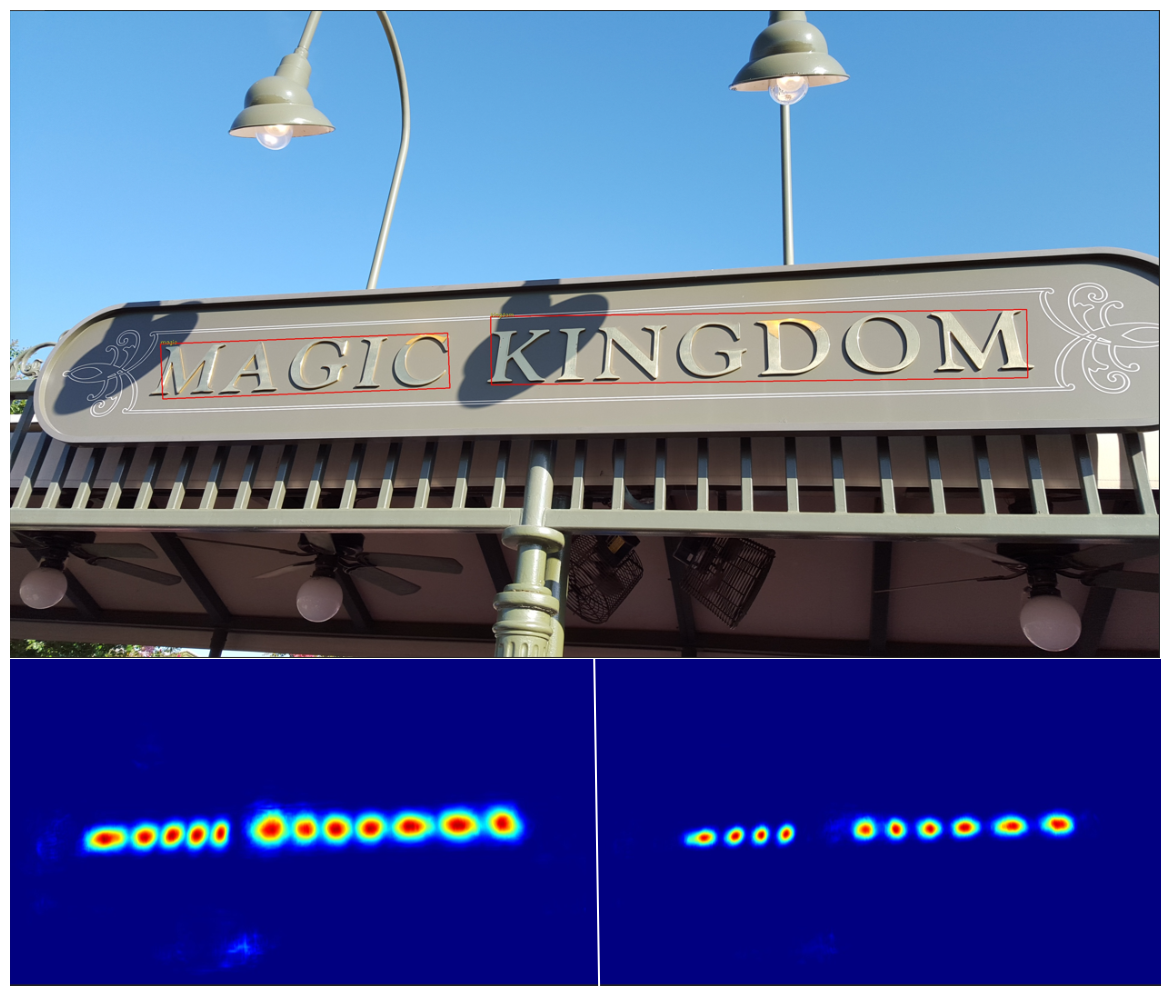
\includegraphics[width=0.8\textwidth]{figs/craft-exmaple.png}
    \caption{Exemplo das imagens geradas a partir da detecção pelo CRAFT sobre uma imagem autoral. Fonte Própria}
    \label{fig:methodology_craft_example}
\end{figure}

Agora sobre o modelo de reconhecimento, para as imagens de entrada, espera-se que contenham apenas uma palavra por imagem e devem respeitar limites de dimensão impostas pela rede que, na implementação utilizada, já são aplicadas durante a execução do \textit{script} de predição, limitando a altura das imagens em 32 pixels. O resultado da predição é a impressão do texto reconhecido ao final da execução do programa. 

A próxima sub-seção abordará, com um pouco mais de detalhes, como as duas soluções escolhidas foram integradas em uma mesma base de código e como os resultados do CRAFT foram processados para que pudessem alimentar a implementação do CRNN, completando a solução fim-a-fim do reconhecimento de texto. 

\section{Desenvolvimento da solução fim-a-fim a partir de detectores e reconhecedores de texto}\label{sec:metodologia_desenvolvimento}

A fim de aplicar o reconhecimento, utilizando o CRNN, exatamente sobre o texto detectado e localizado pelo CRAFT, a escolha foi utilizar o repositório com o código fonte do detector CRAFT como base inicial para a aplicação de reconhecimento fim-a-fim e, a partir dele, adicionar a solução de reconhecimento dentro da mesma base de código e fazer com que ambas tenham todas as dependências necessárias para conseguirem executar seu processamento. Em outras palavras, foi necessário preparar um ambiente de desenvolvimento Python com todas a dependências, a nível de linguagem de programação, bibliotecas e frameworks, instalados e sem conflitos, com tanto as bibliotecas que são dependências obrigatórias para a implementação do CRAFT quanto as bibliotecas que são utilizadas na implementação do CRNN.

Para a gestão de ambientes de desenvolvimento e suas dependências, foi utilizado uma ferramenta no ecossistema Python chamada Conda, mantida pela empresa Anaconda. Com essa ferramenta é possível criar ambientes virtuais Python e instalar todas as dependências necessárias dentro desses ambientes virtuais usando poucas instruções na linha de comando do computador. A própria ferramenta fornece meios para de gerir os ambientes virtuais criados e otimiza a instalação de pacotes dentro desses ambientes de forma que conflitos sejam evitados, resolvendo as versões dos pacotes instalados de forma que sejam compatíveis entre si e compatíveis com a versão da linguagem Python escolhida para o ambiente. Uma grande vantagem de usar esse gerenciados de ambientes Python é a possibilidade de reproduzir qualquer ambiente virtual previamente configurado a partir de um arquivo de configuração, do tipo YAML, que lista todos os pacotes instalados em um ambiente virtual para que, a partir desse arquivo, a ferramenta consiga remontar o mesmo ambiente sem precisar de configurações manuais novamente.

Entrando mais no caminho percorrido para integrar as duas soluções, o primeiro passo foi replicar os repositórios para a conta pessoal do autor no GitHub. Esse processo dentro da plataforma se chama \textit{fork} e em geral é bastante utilizado para possibilitar que outras pessoas consigam desenvolver coisas novas a partir da base de código original sem ter o risco de empurrar mudanças no repositório original inadvertidamente. Dessa forma, ambos os repositórios foram replicados para a conta pessoal do autor e todo o desenvolvimento deste trabalho foi feito nos repositórios replicados.

A partir dos repositórios replicados, foi utilizado um recurso da ferramenta de versionamento, o Git, que possibilita a composição de repositórios a fim de facilitar a sincronização das bases de códigos. O recurso em questão é a criação de sub-módulos em um repositório Git. Usando o comando abaixo a partir do repositório replicado do detector, foi gerado um relacionamento entre as duas bases de código, sendo que o repositório do CRNN agora é visto como um sub-módulo do repositório do CRAFT, e, a partir disso, é possível baixar, usar, evoluir a base de código do repositório do CRNN diretamente do repositório do CRAFT. Isso fez com que ambas soluções já tenham visibilidade uma da outra, mas ainda não fez com que trabalhem juntas.

\begin{minted}{bash}
    git submodule add https://github.com/mmilani1/crnn.pytorch
\end{minted}

Com as soluções na mesma base de código, uma etapa importante é a garantir que ambas ainda funcionam de forma isolada e se validar a compatibilidade das dependências de cada uma. Como mencionado na Seção \ref{sec:metodologia_experimentacao}, uma das motivações da escolha especificamente dessas duas implementações citadas foi justamente a maior proximidade em termos de frameworks e bibliotecas que utilizam, inclusive a possibilidade de ambas soluções poderem ser executadas sem a necessidade de aceleração gráfica. Dessa forma não houveram problemas em executar separadamente cada solução, mesmo compartilhando o mesmo ambiente virtual. O arquivo YAML com a descrição do ambiente virtual pode ser consultado diretamente do repositório com a implementação ou no Apêndice \ref{apd:yaml-desenvolvimento}.

A partir deste ponto já se torna possível trabalhar com os modelos de detecção e reconhecimento a fim de integrá-los, de alguma forma. O objetivo ao fim da integração é conseguir reconhecer texto em imagens de cena, para isso, a ideia é evoluir a extração de resultados do modelo de detecção CRAFT para gerar uma lista de recortes das regiões de texto da imagem original e implementar um algoritmo que execute o modelo de reconhecimento CRNN para cada um desses recortes.

Conforme detalhado na Seção \ref{sec:metodologia_experimentacao}, a implementação do CRAFT fornecida é didática o suficiente com os resultados da detecção, gerando visualizações dos resultados junto com um arquivo de texto contendo as coordenadas das regiões de texto detectadas. Isso demonstra que, em algum ponto do código original as coordenadas dessas regiões de texto foram manuseadas pelos autores do modelo e, consequentemente, poderão ser manuseadas no desenvolvimento da solução integrada a fim de gerar os recortes que serão posteriormente consumidos pelo modelo reconhecimento. O Algoritmo \ref{alg:pseudo_codigo} apresenta o pseudo-algoritmo com as etapas do processamento executado.


\begin{algorithm}
\caption{Pseudo-Código da integração entre a detecção e o reconhecimento de texto}\label{alg:pseudo_codigo}
\begin{algorithmic}
\State $imagem \gets{lerEntrada()}$
\State $palavras \gets{[ ]}$
\State $regioesDeTexto \gets{executaDeteccaoCRAFT(imagem)}$
\For{$regiaoDeTexto \in regioesDeTexto$}
    \State $recorte \gets{recortarTextoDaImagemOriginal(imagem,regiaoDeTexto)}$
    \State $palavra \gets{executaReconhecimentoCRNN(recorte)}$
    \State $palavras \gets{paralvras + [palavra]}$
\EndFor
\State{}
\Return{$palavras$}
\end{algorithmic}
\end{algorithm}

% ```
% imagem = lerEntrada()
% vetoreDePalavrasReconhecidas = []
% vetorDeRegioesDeTexto = detectorCRAFT(imagem)

% para cada regiao em vetorDeRegioesDeTexto:
%   regiaoDeTextoExtraida = extrairRegiaoDaImagemOriginal(regiao)
%   palavra = reconhecimentoCRNN(regiãoDeTextoExtraida)
%   vetorDePalavrasReconhecidas << palavra

% retorna vetorDePalavrasReconhecidas
% ```

Para efetuar o recorte das regiões de texto localizadas e fornecidas na saída do modelo de detecção, foi utilizado um par de funções da biblioteca OpenCV, especializada em ferramentas voltadas para visão computacional. As funções utilizadas foram \texttt{cv2.getPerspectiveTransform} e \texttt{cv2.warpPerspective}.
A primeira função é responsável por gerar uma matriz de transformação de áreas quadrangulares e recebe duas sequencias de pontos. A primeira sequência contém os vértices da área quadrangular a ser transformada, no caso desse trabalho, são as coordenadas da \textit{bounding-box} de uma palavra detectada. Já a segunda sequência de pontos representa os vértices da imagem de saída, para onde o cada um dos pontos da primeira sequência serão transportados após a aplicação da transformação.
A segunda função é responsável por aplicar a matriz de transformação, gerada a partir da execução do comando \texttt{cv2.getPerspectiveTransform}, sobre a imagem onde o texto foi detectado. Dessa forma conseguimos recortar as palavras detectadas da imagem original de forma cada é possível posteriormente passar as referências desses recortes para o modelo de reconhecimento diretamente, já que a os dados de entrada esperados pelo CRNN são imagens que contém idealmente uma palavra para reconhecimento. A Figura \ref{fig:methodology_pipeline} ilustra, em alto nível, as etapas do processamento que compõem as solução de STR fim-a-fim deste trabalho.

\begin{figure}
    \centering
    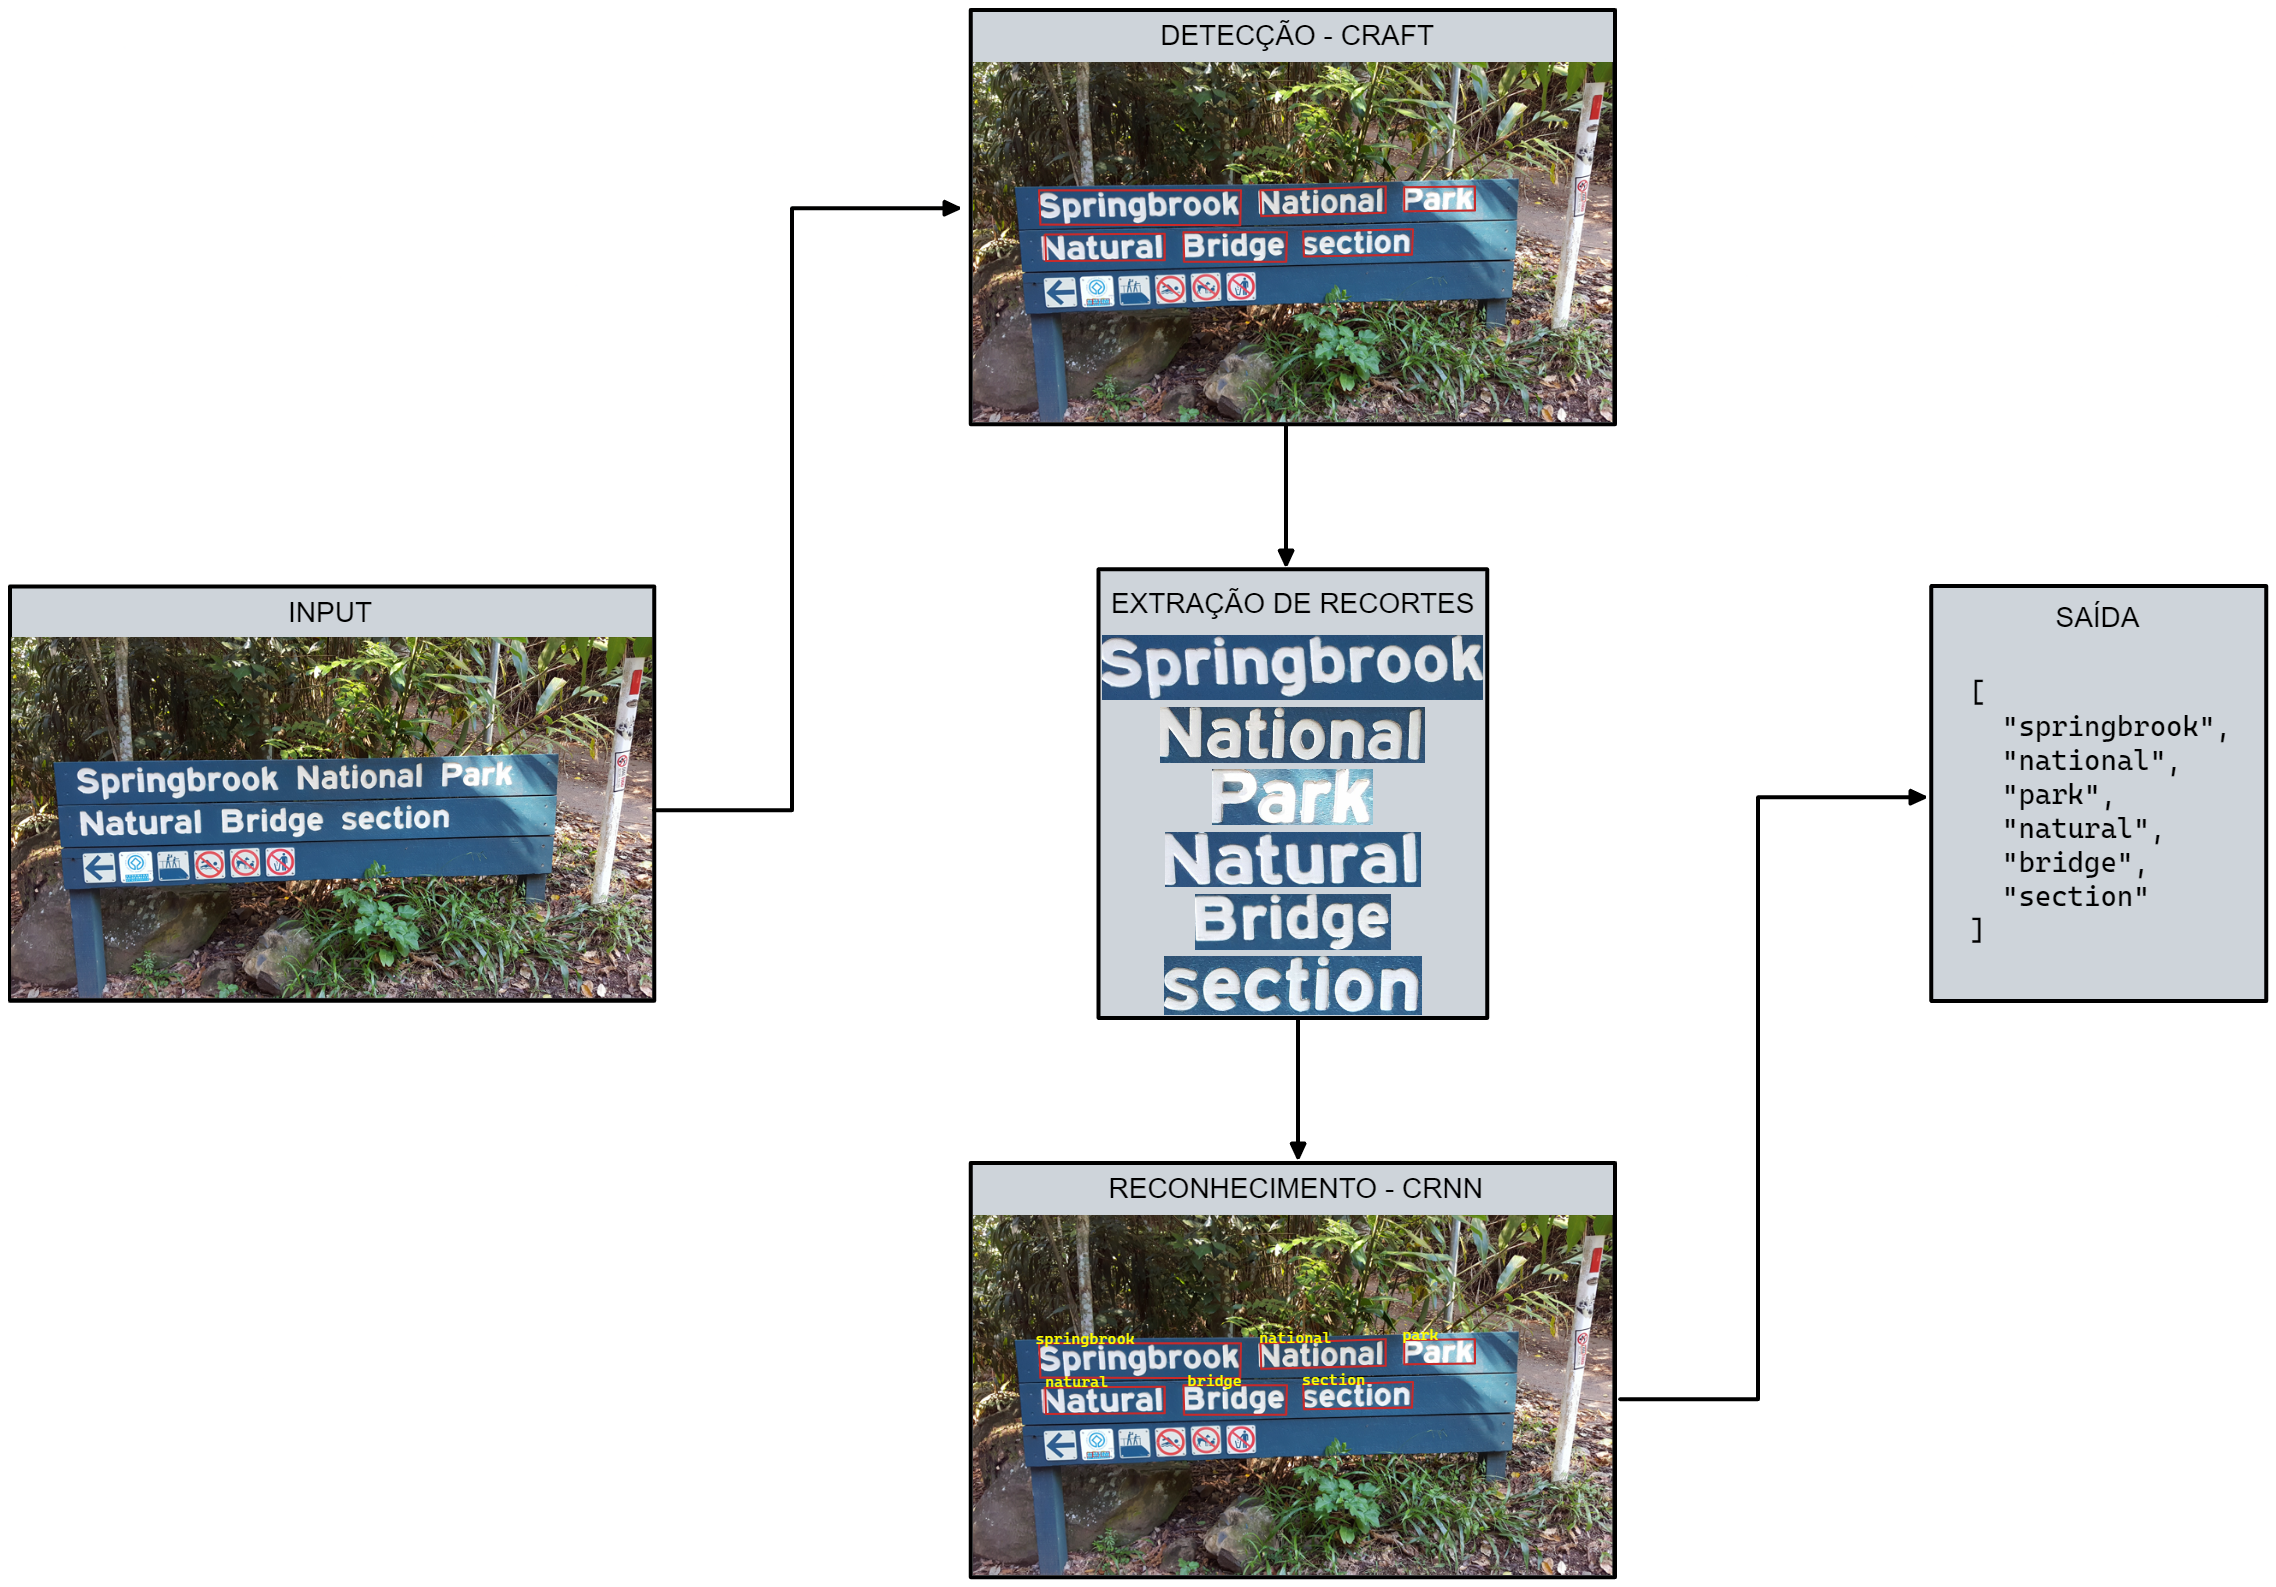
\includegraphics[width=0.8\textwidth]{figs/metodologia-pipeline.png}
    \caption{Ilustração das etapas de processamento da solução proposta. Fonte Própria}
    \label{fig:methodology_pipeline}
\end{figure}

Ao fim dessas alterações, integrando os dois modelos de detecção e reconhecimento, já temos uma solução simples de reconhecimento de texto em cenas que pode ser classificada como \textit{end-to-end}, que contempla tanto a detecção quanto o reconhecimento dentro de uma mesma aplicação. A próxima etapa é conseguir avaliar a eficácia desse novo desenvolvimento. A próxima seção introduzirá os métodos e métricas utilizadas para avaliar a solução.

\section{Método de avaliação da solução proposta}\label{sec:methodology_validation}

A avaliação analítica da solução proposta neste trabalho é baseada na forma de avaliação da plataforma \textit{Robust Reading Competition} (abreviação RRC), disponibilizado pelo Centro de Visão Computacional da Universidade Autônoma de Barcelona. Essa plataforma organiza competições em torno de problemas reais de visão computacional e tipicamente essas competições se relacionam com a Conferência Internacional sobre Análise e Reconhecimento de Documentos, abreviada como ICDAR, a partir no nome da conferência em inglês. Diversos datasets que são amplamente adotados para treino e avaliação de modelos de reconhecimento de texto levam no nome a menção ao ICDAR, por introduzirem a base da dados e os desafios propostos, fomentando novos trabalhos na área.

Essa seção irá introduzir dos datasets avaliados, as métricas utilizadas e o processo de avaliação da solução apresentada utilizando as ferramentas de avaliação disponibilizadas pela plataforma RRC.

\subsection{Datasets}\label{sec:methodology_datasets}

Conforme mencionado anteriormente, os datasets dos desafios vinculados ao ICDAR são muito utilizados por trabalhos voltados à detecção e reconhecimento de texto. Ambos os modelos utilizados no desenvolvimento deste trabalho fazem referência aos datasets ICDAR: O CRAFT cita os datasets ICDAR 2013, ICDAR 2015 e ICDAR 2017 como bases de treinamento e de validação em quanto o CRNN se refere ao ICDAR 2003 e ICDAR 2013 como bases de imagens para validação. Os datasets utilizados para a avaliação deste trabalho foram o ICDAR 2011, base para o primeiro desafio da platafoma RRC chamado \textit{Reading Text in Born-Digital Images}, e o ICDAR 2013, que é a base para o segundo desafio da plataforma RRC, chamado \textit{Focused Scene Text}.

\subsubsection{ICDAR 2011}\label{sec:datasets_icdar2011}
O ICDAR 2011 conta com 410 imagens para treino e 141 imagens para validação, imagens que estão no contexto de anúncios de internet e anexos de e-mails, com palavras em geral na horizontal e anotadas com \textit{bounding-boxes} retangulares a nível de palavras. As imagens são anotadas com a localização de cada palavra com coordenadas das \textit{bounding-boxes} retangulares, que servem como gabarito para soluções de detecção e localização. Cada imagem também conta com a transição das palavras para servir como gabarito de soluções de reconhecimento conta A Figura \ref{fig:icdar2011_examples} expõe algumas imagens deste dataset.

\begin{figure}
    \centering
    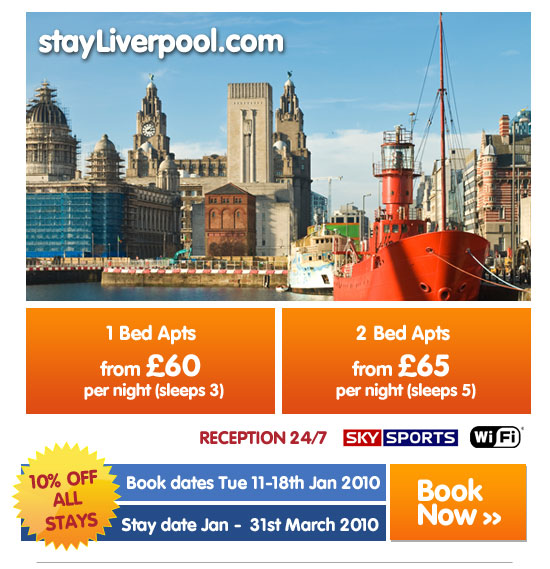
\includegraphics[width=0.3\textwidth]{figs/img_33.png}
    
\includegraphics[width=0.3\textwidth]{figs/img_62.jpg}
    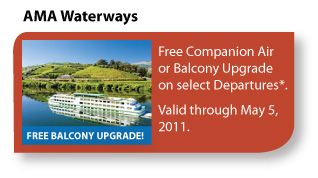
\includegraphics[width=0.3\textwidth]{figs/img_13.jpg}
    \caption{Exmplos de imagens do dataset ICDAR 2011. Fonte [\citeonline{ICDAR2011}]}
        \label{fig:icdar2011_examples}
\end{figure}

\subsubsection{ICDAR 2013}\label{sec:datasets_icdar2013}
O ICDAR 2013 conta com 219 imagens para treino e 233 imagens para validação . São imagens de cenas onde em geral o texto tem boa qualidade e está em destaque, na orientação horizontal. As anotações de gabarito são retangulares a nível de palavras e contam com a transição das mesmas, de forma similar às imagens do ICDAR 2011. A Figura \ref{fig:icdar2013_examples} expõe algumas imagens deste dataset.

\begin{figure}
    \centering
    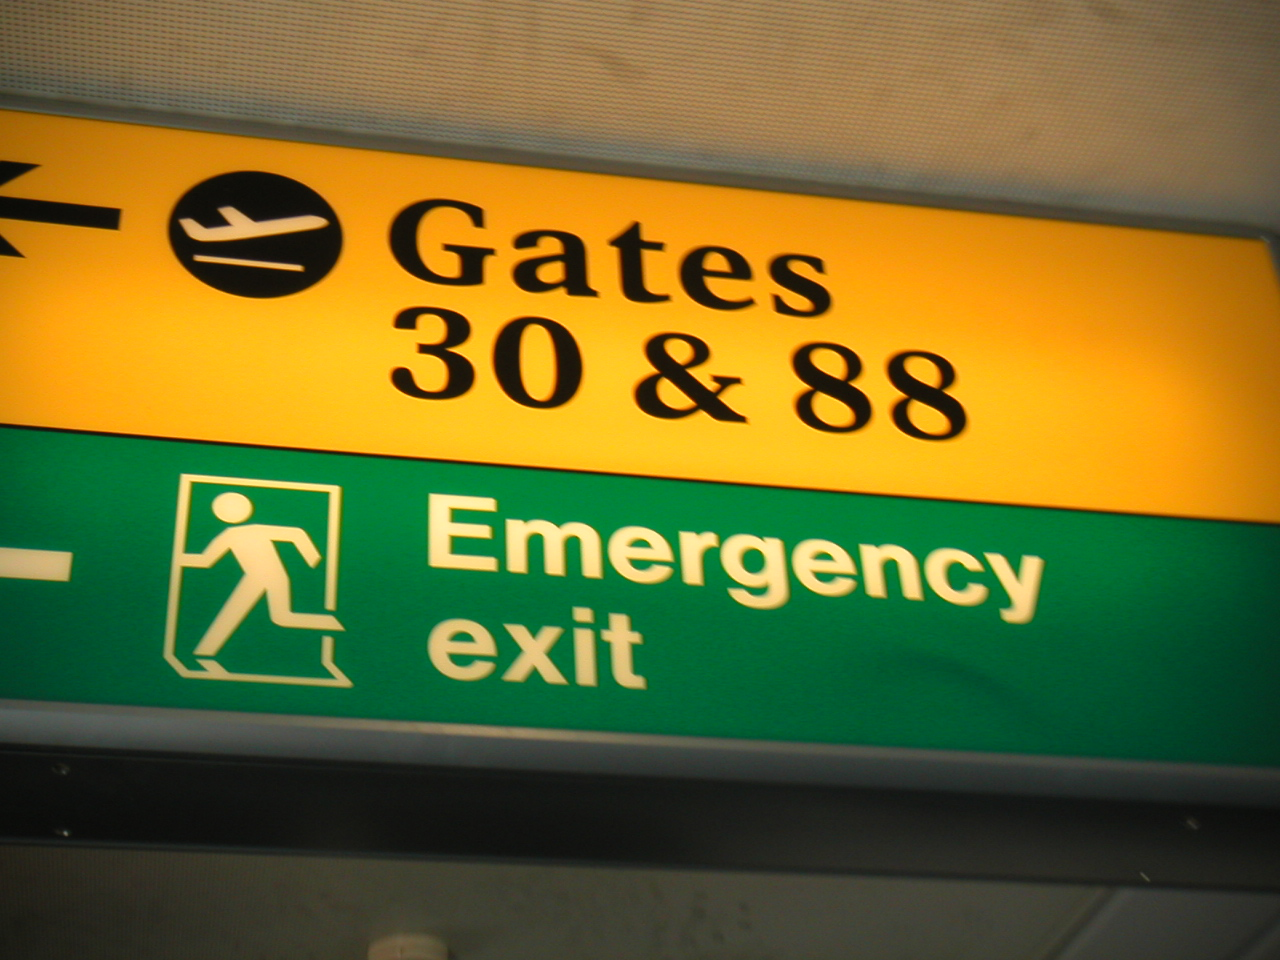
\includegraphics[width=0.3\textwidth]{figs/img_20.jpg}
    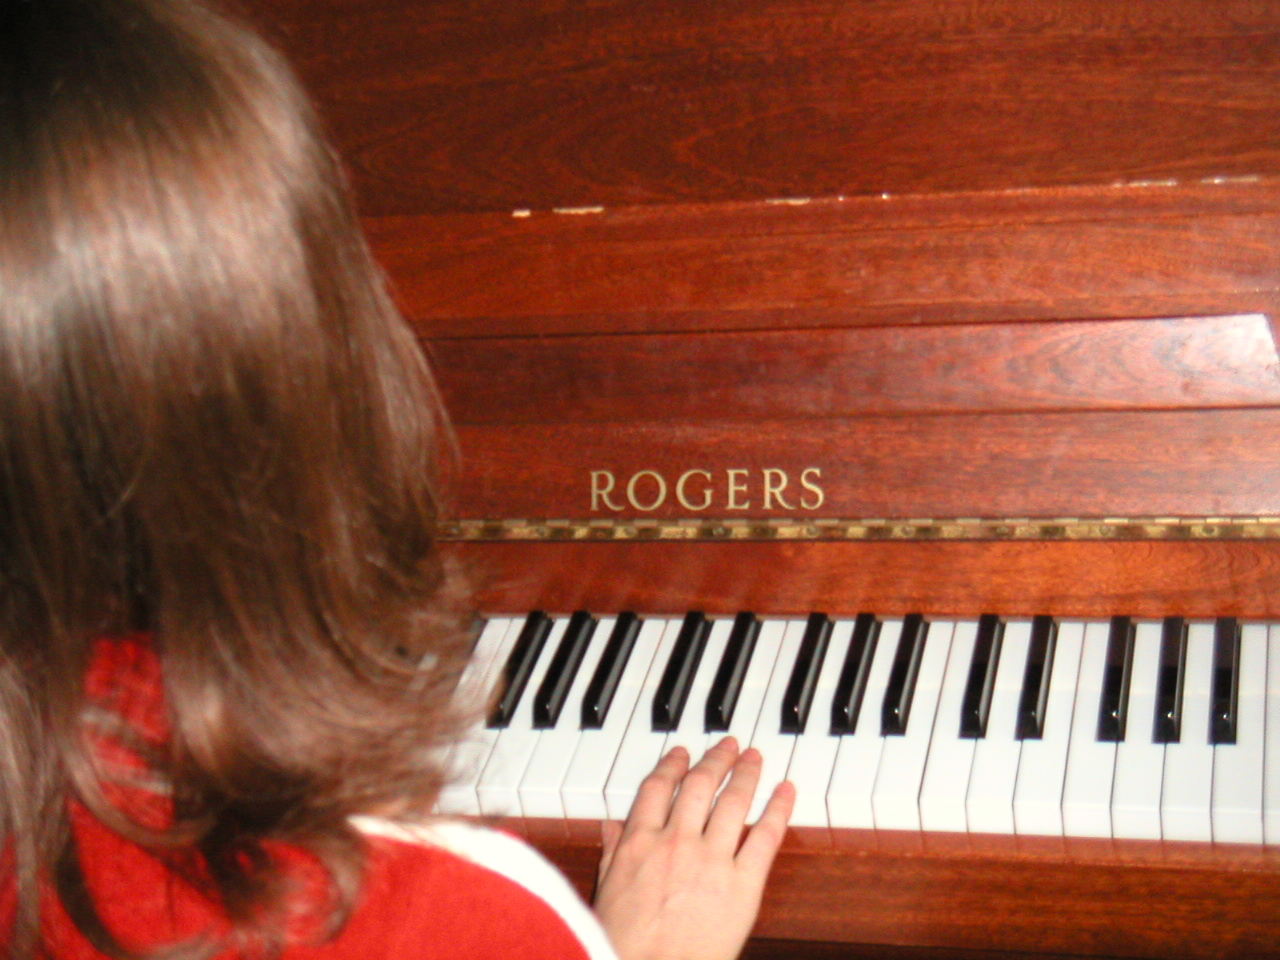
\includegraphics[width=0.3\textwidth]{figs/img_85.jpg}
    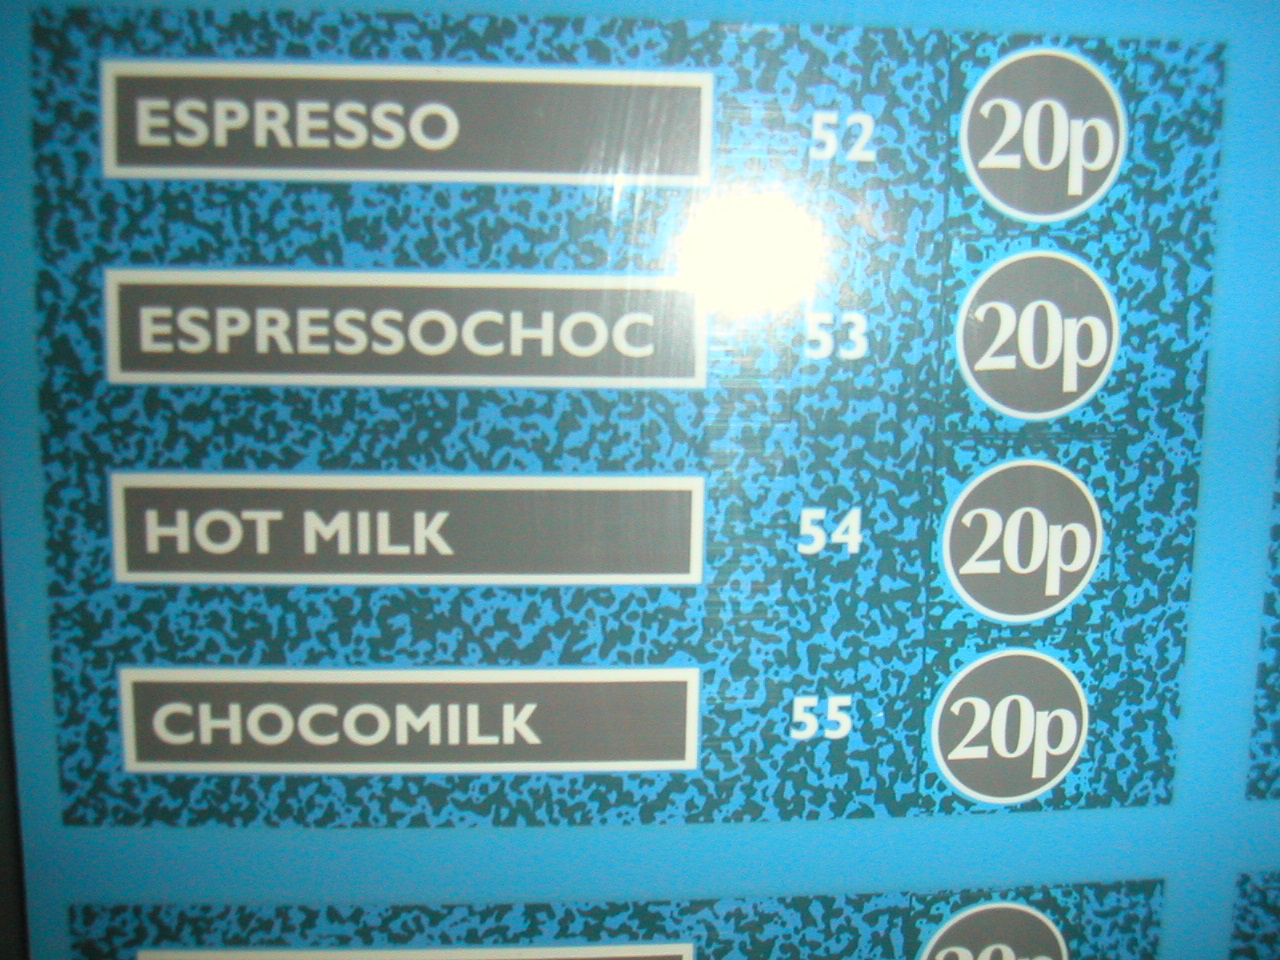
\includegraphics[width=0.3\textwidth]{figs/img_225.jpg}
    \caption{Exmplos de imagens do dataset ICDAR 2013. Fonte [\citeonline{ICDAR2013}]}
    \label{fig:icdar2013_examples}
\end{figure}

\subsection{Métricas}\label{sec:methodology_metrics}
Em conjunto aos datasets, são fornecidas meios de avaliação para que cada nova solução que surgir possam ser avaliadas sob os mesmos termos, usando os mesmos conceitos e as mesmas métricas. Na plataforma RCC e nos datasets que eles disponibilizam são utilizados: Precisão, Recall e F1-Score (ou H-Mean). A Precisão é a relação dos acertos (verdadeiros positivos) sobre a contagem total de predições positivas (verdadeiros positivos e falsos negativos), ou seja, dentre as predições da solução, qual é a porcentagem de acerto. O Recall relaciona a quantidade de acertos com a quantidade total de casos verdadeiros. O F1-Score é basicamente a média harmônica das métricas Precisão e Recall.

\begin{equation}
    Precisão = \frac{VP}{VP + FP}
\end{equation}
\begin{equation}
    Recall = \frac{VP}{VP + FN}
\end{equation}
\begin{equation}
    F1Score = 2 \times \frac{Precisão \times Recall}{Precisão + Recall}
\end{equation}

Para determinar se uma predição foi correta existem duas condições: A região de texto detectada deve satisfazer uma métrica característica de eficácia em detecção e localização das palavras na imagem chamada IoU, abreviação para \textit{Intersection over Union}, além da transcrição predita ser exatamente igual ao gabarito. Para uma predição ser considerada correta, o valor de IoU, que se resume à precisão da detecção, deve ser maior ou igual a 50\%.

A métrica de IoU pode ser calculada a partir das coordenadas verdadeiras de uma região de texto, documentadas nas anotações dos datasets, e das coordenadas preditas pelo modelo de detecção. Ambos conjuntos de coordenadas descrevem uma área retangular, para os dois datasets utilizados. Com esses dois conjuntos de valores, pode-se avaliar tanto o tamanho da intersecção entre a área predita e a área esperada, quanto o tamanho da união entre ambas as áreas. O valor numérico da métrica IoU decorre, conforme sugerido pelo nome da métrica, da divisão entre o tamanho da intersecção sobre o tamanho da união entre as áreas preditas e as áreas esperadas.

\subsection{Interface de Validação}\label{sec:methodology_validation_interface}
Na plataforma do RRC é possível avaliar uma solução formalizando a submissão dos resultados diretamente no site da competição, dessa forma os resultados ficam registrados na plataforma e pode ser até ranqueada junto a outros trabalhos submetidos. Para cada desafio da plataforma existe o ranque de soluções, onde é pode-se observar resultados de outros trabalhos de maneira simples e, quando disponível, até consultar quem são os autores, se existe algum repositório publico para a base de código, visualizar o artigo do trabalho, etc.

No entanto não é a única opção. Existe a opção de efetuar o download dos \textit{scripts} que calculam os resultados, nos mesmos moldes da avaliação remota, a fim de executar todo o processo localmente, que foi o método adotado para esse trabalho.

Para ambos os meios de validação, é necessário preparar arquivos de resultados, para cada imagem do dataset de validação, com os dados necessários para a avaliação. Tanto o ICDAR 2011 quanto o ICDAR 2013 demandam arquivos com o mesmo formato, que se assemelham justamente aos arquivos de gabarito dessas bases, e seguem o seguinte formato descrito abaixo. Um exemplo de arquivo de resultado foi disponibilizado no Apêndice \ref{apd:exe_resultado}

\begin{itemize}
    \item É necessário gerar um arquivo de texto, para cada imagem, nomeados respeitando o seguinte formato: \texttt{res\_img\_\#.txt}, onde o \texttt{\#} corresponde ao identificador numérico da imagem no dataset.
    \item Cada arquivo deve ter uma linha para cada palavra detectada e reconhecida.
    \item Cada linha deve conter os seguintes valores, separados por virgula simples, exatamente na ordem especificada: posição do vértice esquerdo superior da bounding-box, vértice direto inferior da bounding-box e texto da transição.
\end{itemize}

Após gerar todos os arquivos necessários, resta agregá-los em um arquivo comprimido do tipo ZIP e, ou submeter a solução diretamente na plataforma da competição, ou executar a ferramenta de validação localmente. Os arquivos de execução local são escritos em Python e dependem de poucas bibliotecas. Executam um leve servidor web para servir a aplicação de validação. Durante a execução da validação deste trabalho, foi utilizado novamente a ferramenta Conda para gerir essas dependências. O Apêndice \ref{apd:yaml-validacao} contém o arquivo que descreve o ambiente virtual utilizado. A Figura \ref{fig:methodology_validation_interface} mostra um pouco da interface de usuário que a a aplicação fornece, com as funcionalidades de submeter o arquivo comprimido de solução e a Figura \ref{fig:methodology_validation_interface_details} mostra a funcionalidade de verificação dos resultados sobre cada imagem, possibilitando a análise sobre onde as soluções funcionaram bem e onde não funcionaram tão bem, o que foi feito no contexto da solução proposta nesse trabalho no Capitulo \ref{cap:resultados}.

\begin{figure}
    \centering
    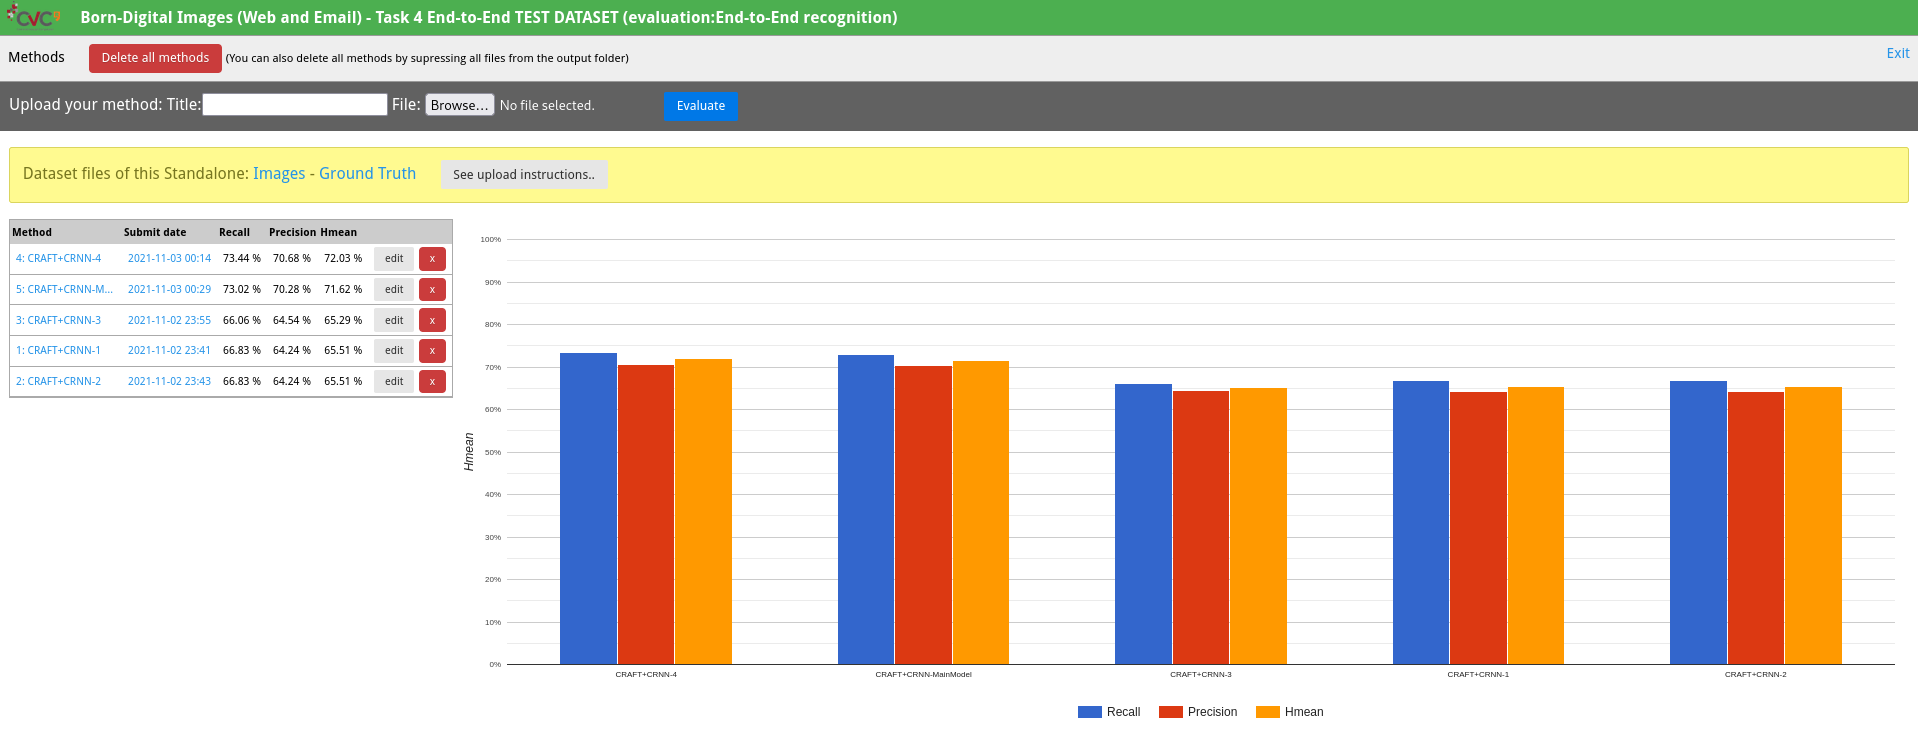
\includegraphics[width=0.8\textwidth]{figs/metodologia-interface-validacao.png}
    \caption{Interface de validação disponibilizada pela plataforma de desafios Robust Reading Competition. Fonte Própria}
    \label{fig:methodology_validation_interface}
\end{figure}

\begin{figure}
    \centering
    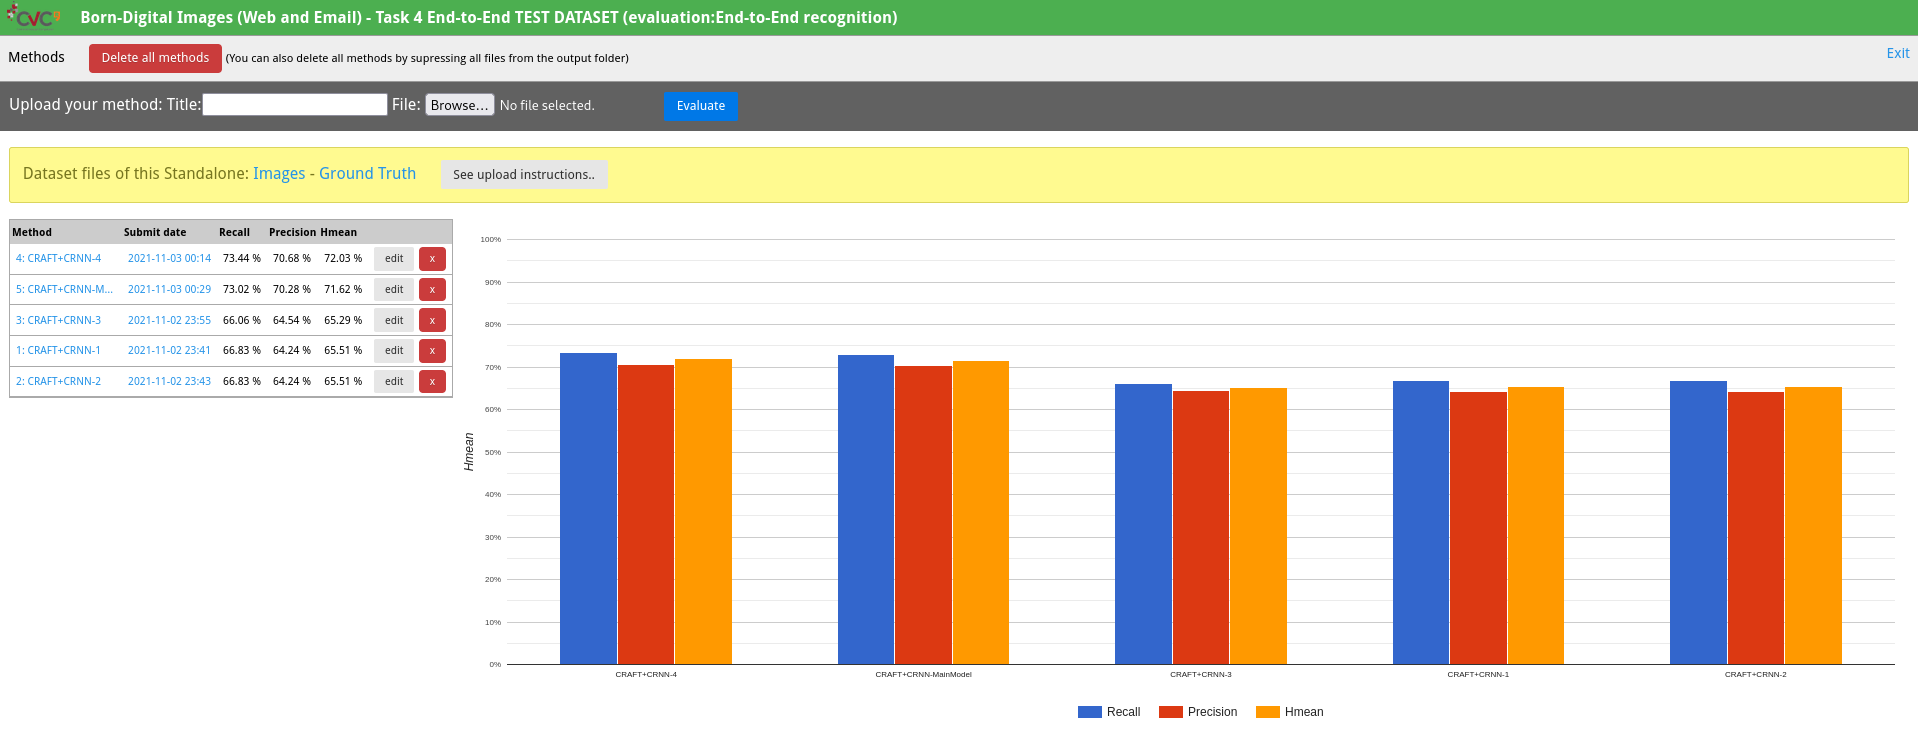
\includegraphics[width=0.8\textwidth]{figs/metodologia-interface-validacao.png}
    \caption{Interface de validação disponibilizada pela plataforma de desafios Robust Reading Competition, com visualização de detalhes da avaliação por imagem. Fonte Própria}
    \label{fig:methodology_validation_interface_details}
\end{figure}

\section{Disponibilização da solução fim-a-fim em nuvem}\label{sec:methodology_cloud_deploy}
Uma vez com o desenvolvimento da integração entre os componentes concluída e avaliada, a próxima etapa para atingir os objetivos deste trabalho de graduação é executar uma prova de conceito sobre a solução proposta e disponibilizá-la em como uma aplicação web, hospedada em nuvem, assim possibilitando demonstrar que seria possível distribuir a funcionalidade para outros, possivelmente até evoluir para um serviço digital de reconhecimento de texto, vendido como produto.

Existem diversas provedoras de computação em nuvem que poderiam ser utilizadas, entre as mais notáveis estão a gigante AWS (Amazon Web Services) e a a própria Paperspace, utilizada sob-demanda por esse trabalho durante o desenvolvimento conforme citado na Seção \ref{sec:metodologia_experimentacao}. Ambas teriam infraestrutura para comportar a solução proposta por este trabalho, inclusive provendo máquinas com alto poder computacional dependendo da necessidade e dos limites financeiros do projeto. Como ambos serviços, apesar de possuírem limites de uso onde os recursos são gratuitos, não são de domínio do autor deste trabalho de graduação. Como uma terceira terceira opção, a plataforma escolhida para hospedar o desenvolvimento deste trabalho foi o Heroku. No entanto, mesmo tendo escolhido uma plataforma especifica para hospedar a aplicação, as ferramentas e o processo até a publicação em geral são parecidas, então, resguardadas as devidas proporções, o processo feito para publicar a aplicação no Heroku pode ser extrapolado para algo similar em outras provedores de infraestrutura.

O Heroku uma plataforma disponibilizada pela empresa Salesforce que age como uma camada de abstração sobre os provedores de nuvem e seus componentes de mais baixo nível, justamente para prover uma interface mais simples, facilitando a gestão de infraestrutura para desenvolvedores. As etapas para publicar uma aplicação para o Heroku envolvem poucos comandos e também existe a possibilidade de hospedar aplicações usando recursos gratuitos. As limitações do ambiente gratuito e suas implicações na execução da aplicação serão abordadas no Capítulo \ref{cap:resultados}

\subsection{Criação da Aplicação Web}\label{sec:methodology_web_app}
Até então, tudo que foi desenvolvido para este trabalho foi executado interagindo diretamente com os componentes da base de código, executando os \textit{scripts} de detecção e reconhecimento através de uma linha de comando. Para expor o modelo integrado para na internet, a ideia foi criar uma aplicação web, nos moldes de cliente-servidor, que responde requisições pelo protocolo HTTP, utilizando a arquitetura REST. Para isso foi necessário fazer algumas adições à base de código para contemplar a implementação de uma aplicação web utilizando o framework Flask, que permite, com pouquíssima configuração, executar um servidor HTTP e possibilita que uma requisição seja atendida por um método da base de código.

Como o código existente esperava ser executado através dos \textit{scripts} diretamente, dependendo de parâmetros de linha de comando por exemplo, foi necessário a criação de um novo arquivo contendo uma classe Python que centralizasse a execução dos métodos necessários para o funcionamento do reconhecimento fim-a-fim. Essa classe foi denominada \texttt{OcrRunner} e centraliza toda a orquestração do processamento, desde a preparação dos modelos junto ao framework PyTorch, até a execução de fato da detecção e do reconhecimento de forma integrada. Com isso, foi possível executar a solução fim-a-fim programaticamente.

Além da nova classe implementada, foi necessário criar um novo método que tem a responsabilidade atender a requisição originada pelo cliente. Esse método, com a ajuda do framework Flask, consegue receber um arquivo de imagem enviado pelo cliente e executar a solução proposta sobre a imagem enviada. Por fim, quando o reconhecimento termina, o retorno do método é a lista de palavras reconhecidas, que, automaticamente, é respondido ao cliente que fez a requisição.

Com essas poucas mudanças já é possível, de maneira miníma e muito simplificada, atender pedidos de reconhecimento de texto sob demanda. O próximo passo adotado foi utilizar ferramentas e conceitos voltados a conteinerização da aplicação para facilitar a execução no ambiente remoto.

\subsection{Contêiner, Docker e Publicação}
Uma prática muito usual ao utilizar a computação em nuvem como meio de hospedar aplicações é gerar arquivos executáveis contendo tudo o que a aplicação precisa para funcionar: A base de código, as dependências, os binários, as configurações e tudo mais que for necessário, de maneira consistente e de fácil reprodutibilidade. Esse processo é por vezes chamado de conteinerização, onde um contêiner é esse agregado do código da aplicação e tudo o que for necessário para executá-la, de fato sendo executado. Uma das tecnologias de contêiner mais utilizadas é o Docker [\citeonline{Docker}]. Mais detalhes sobre Docker e contêineres podem ser encontrados na página oficial da tecnologia.

A fim de gerar um contêiner da aplicação desenvolvida neste trabalho, o primeiro passo foi descrever como esse contêiner é construído, e, para isso, cria-se um arquivo chamado de Dockerfile. Nele consta uma série de comandos que são executados rigorosamente pelo Docker para criar uma imagem Docker. Ao executar a imagem pelo Docker, um contêiner é inicializado com o conteúdo da imagem executada e pode executar o código que foi compilado na imagem Docker. O arquivo Dockerfile pode ser consultado diretamente no repositório desse trabalho ou no Apêndice \ref{apd:dockerfile}.

Ter a aplicação "conteinerizada" economiza muita configuração na hora de publicá-la na nuvem, já que não se faz mas necessário configurar o servidor onde a aplicação será servida de forma especifica para satisfazer as demandas de binários e bibliotecas para a aplicação em questão. Tudo o que é necessário para executar a aplicação já está definido na imagem do contêiner e estará pronto pra uso quando o contêiner foi iniciado, dessa forma, as etapas mencionadas nas Seções \ref{sec:metodologia_experimentacao} e \ref{sec:metodologia_desenvolvimento} referentes a configuração do ambiente Python e instalação de dependências através do Conda já foi resolvido na criação da imagem e o ambiente já estará pronto para uso dentro do contêiner. O servidor que hospeda os contêineres não precisa saber de especificidades de cada aplicação, sua responsabilidade é saber executar os contêineres e compartilhar recursos computacionais com eles. Dessa forma, a publicação da aplicação no Heroku se resume a execução de um comando a interface de linha de comando que a plataforma disponibiliza para publicar uma aplicação a partir de uma imagem Docker.

\section{Considerações finais}
De forma sucinta, nesse capitulo foi apresentado como ocorreu o desenvolvimento deste trabalho de graduação, mencionando como os modelos de detecção e reconhecimento foram escolhidos, como e com quais ferramentas eles foram testados, integrados e, ao final da integração como a solução foi validada e publicada em nuvem.

O próximo capitulo abordará mais a fundo os resultados do desenvolvimento, com enfoque na capacidade de detecção e reconhecimento do modelo integrado e discutindo um pouco sobre a execução da aplicação em nuvem.